% !TeX encoding = UTF-8
% !TeX program = xelatex
% !TeX spellcheck = en_US

\documentclass{cjc}

\usepackage{booktabs}
\usepackage{algorithm}
\usepackage{algorithmic}
\usepackage{siunitx}

\classsetup{
  % 配置里面不要出现空行
  title        = {基于Conditional Gated PixelCNN的图像超分辨率重建},
  title*       = {Image Super Resolution Reconstruction based on Conditional Gated PixelCNN},
  authors      = {
    author1 = {
      name         = {刘羿},
      name*        = {Yi Liu},
      affiliations = {aff1},
      biography    = {种子1701班,U201713371,主要研究领域为网络安全},
      % 英文作者介绍内容包括:出生年, 学位(或目前学历), 职称, 主要研究领域(与中文作者介绍中的研究方向一致).
      biography*   = {SeedClass 1701, U201713371,His research interests lie within Cyber security},
      email        = {liuyi12138@hust.edu.cn},
      phone-number = {18627746983},  % 第1作者手机号码(投稿时必须提供,以便紧急联系,发表时会删除)
    },
    author2 = {
      name         = {张志宇},
      name*        = {Zhiyu Zhang},
      affiliations = {aff1},
      biography    = {种子1701班,U201710997,,主要研究领域为网络安全、网络通信和机器学习.},
      biography*   = {SeedClass 1701, U201710997, His research interests lie within Cybersecurity, Network Communications and Machin Learning},
      email        = {zhiyuzhang@hust.edu.cn},
    },
    author3 = {
      name         = {李勉},
      name*        = {Mian Li},
      affiliations = {aff1},
      biography    = {种子1701班,U201712070,主要研究领域为网络安全.},
      biography*   = {SeedClass 1701, U201712070, His research interests lie within Cybersecurity},
      email        = {1350747952@qq.com},
      % 通讯作者
    %   corresponding = true,
    },
  },
  % 论文定稿后,作者署名、单位无特殊情况不能变更。若变更,须提交签章申请,
  % 国家名为中国可以不写,省会城市不写省的名称,其他国家必须写国家名。
  affiliations = {
    aff1 = {
      name  = {华中科技大学\ 电子信息与通信学院, 武汉市, 中国\ 430074},
      name* = {Department of Electronic Information and Communications, Huazhong University of Science and Technology, 430074, China},
    },
  },
  abstract     = {
    % 中文摘要内容置于此处(英文摘要中要有这些内容),字体为小5号宋体。
    % 摘要贡献部分,要有数据支持,不要出现“...大大提高”、“...显著改善”等描述,
    % 正确的描述是“比…提高 X\%”、 “在…上改善 X\%”。
    图像的超分辨率重建是人为地通过数字图像处理等方法将低分辨率的图像重建为高分辨率图像的过程。基于传统图像插值的重建方法难以构建输入输出的非线性依赖关系,而基于生成对抗网络的方法难以克服模式崩溃和数据多样性缺乏的问题,因此我们提出了基于条件的门限PixelCNN网络,它能够以递归的形式将图像的先验信息以条件的形式来限制CNN预测网络,从而达到很好的超分辨率重建效果。本文以亚洲人脸为重点实验对象,最终实现将16x16的低分图像较完美的生成64x64的高分图像,并对于非人脸图像具有良好的可迁移性。
  },
  abstract*    = {Abstract 
Image super-resolution reconstruction is a process of artificially reconstructing low-resolution images into high-resolution images through digital image processing methods. The reconstruction based on traditional image interpolation is difficult to construct the non-linear dependence of input and output, and the method based on generating adversarial network is difficult to overcome the problems of mode collapse and lack of data diversity. Therefore, we propose a Conditional Gated PixelCNN network, which can recursively input the prior information of the image as a condition to limit the CNN prediction network, so as to achieve a great super-resolution reconstruction effect. This paper focuses on Asian faces reconstruction, and finally achieves a perfect rebuilding from 16x16 LR image to 64x64 HR image, which also own a good portability in other types of images. },
  % 中文关键字与英文关键字对应且一致,应有5-7个关键词,不要用英文缩写
  keywords     = {图像超分辨率重建, PixelCNN, 先验条件限制},
  keywords*    = {Image Super-resolution Reconstruction, PixelCNN, Prior Conditional Limit, },
  grants       = {
    三位作者为并列第一作者,作者信息如下:
  },
  % clc           = {TP393},
  % doi           = {10.11897/SP.J.1016.2020.00001},  % 投稿时不提供DOI号
  % received-date = {2019-08-10},  % 收稿日期
  % revised-date  = {2019-10-19},  % 最终修改稿收到日期,投稿时不填写此项
  % publish-date  = {2020-03-16},  % 出版日期
  % page          = 512,
}

\newcommand\dif{\mathop{}\!\mathrm{d}}

% hyperref 总是在导言区的最后加载
\usepackage{hyperref}



\begin{document}

\maketitle


\section{引言}
随着科学研究和技术的不断推进,我们已经进入了一个信息爆炸的时代。而图像是人们从客观世界获取信息的重要来源,因为人类是通过感觉器官从客观世界获取信息的,即通过耳、目、口、鼻、手通过听、看、味、嗅和接触的方式获取信息,而在这些信息中视觉信息占据70\%\cite{zhy2007review}。因此数字图像处理在通信领域和计算机视觉领域占据了举足轻重的地位。

在大量的数字图像应用领域,人们经常期望得到高分辨率(简称HR)图像。但受限制于设备,传感器亦或者信道干扰等因素,我们得到的图像往往是低分辨率图像(LR)。增加空间分辨率最直接的解决方法就是通过传感器制造技术减少像素尺寸(例如增加每单元面积的像素数量);另外一个增加空间分辨率的方法是增加芯片的尺寸,从而增加图像的容量。因为很难提高大容量的偶合转换率,所以这种方法一般不认为是有效的,因此,引出了图像超分辨率重建技术。

超分辨率图像重建(Super resolution image re-construction, SRIR或SR)是指用信号处理和图像处理的方法,通过软件算法的方式将已有的低分辨率(Low-resolution, LR)图像转换成高分辨率(High-resolution, HR)图像的技术.它在视频监控(Video surveillance)、图像打印(Image printing)、刑侦分析(Criminal investigation analysis)、医学图像处理(Medical image processing)、卫星成像(Satellite imaging)等领域有较广泛的应用\cite{Su2013review}. 

因此本文以图像的超分辨率重建为研究目标,提出了一种基于Conditional Gated PixelCNN的方法实现针对低分辨率的人脸图像的超分辨率恢复。本文首先介绍了研究的背景,接着讨论了相关领域前人的工作,然后提出了我们基于Conditional Gated PixeCNN的算法设计及其改进,设计并展示了相应的对比实验和结果,最终我们将讨论我们的研究结果并总结我们的工作。

\section{相关工作}
在上世纪80∼90年代,就有人开始研究超分辨率图像重建的方法,1984年Tsai的论文\cite{tsai1984multiframe}是最早提出这个问题的文献之一. 1998年, Borman等\cite{borman1998spatial}发表了一篇超分辨率图像重建的综述文章. 2003年, IEEE Signal Processing Magazine发布了一期超分辨率图像重建的专刊\cite{park2003super}. 这些较早期的综述文章主要介绍传统的基于重建的超分辨率算法的研究情况.

而近年来,关于图像超分辨率的重建的研究逐渐出现明确的方向分化,其中针对单一图像的超分辨率重建的研究可以分为无训练样本的增强边缘的单帧超分辨率研究和有训练样本的基于学习的单帧超分辨率研究\cite{Su2013review}。无训练样本的增强边缘超分辨率重建本质上其实是对图像边缘信息的增强处理,主要通过传统图像插值技术。但是由于线性模型无法表达输入和输出之间的复杂依赖关系,因此这些方法由于缺乏可表达性而受到困扰。在实践中,此类方法通常无法充分预测高频细节,从而导致高分辨率输出模糊。基于学习的方法在单帧图像超分辨率重建领域里表现出色。它们采用机器学习方法从大量训练样本中提取图像的高频特征,并构建映射模型,从而对未知测试样本图像的信息进行预测,达到提高图像分辨率的目的。

CNN是很好一种提取图像信息的网络结构,董等人\cite{dong2015image}采用了以MSE损失为度量的三层CNN实现了低分辨率到高分辨率的初步映射,而Kim等人\cite{kim2016accurate}通过将深度提高到了20层并仅学习高分辨率图像和插值的低分辨率图像的残差,从而提高了精度。陈等人\cite{Chen2020Res}使用了具有更大感受野的深层残差网络,并引入局部残差学习和全局残差学习相结合的方法来提高学习率,与现有的Bicubic和SRCNN相比重建效果得到了提升。

此外,采用对抗损失才训练网络也是一个很好的超分辨率重建的研究方向。Metz等人\cite{metz2016unrolled}介绍了一种通过定义针对鉴别器的展开优化的生成器目标来稳定生成对抗网络的方法,从而实现有效的防止模式崩溃和数据多样性缺乏的问题。Ledig等人\cite{ledig2017photo}提出了用于图像超分辨率的网络SRGAN,使用感知相似性而非像素空间相似性引起的内容损失作为损失度量,实现了以4倍为因子的像素放大。

然而基于CNN的网络模型无法很好的修补超分辨率的图像细节,而基于GAN的网络模型常常面临无法覆盖到数据样本的多样性的问题。针对GAN的现存问题,我们寻找到了一种基于PixelCNN的先验概率生成模型\cite{oord2016pixel,van2016conditional},它能够有效地处理与给定低分辨率图像相关联的高分辨率图像的多样性。我们还将PixelCNN与CNN网络进行结合,从而有效解决了图像重建的细节修复问题。

% \newpage
\section{算法原理}
\subsection{模型基本结构}

本论文采用的图像超分辨率重建的方法,采用了一个被称为Conditional Gated PixelCNN的图像处理模型。我们的模型可以在逻辑上分为两部分,一部分被称为Conditioning network,另一部分为Prior network。

Conditioning network是一个预测模型,其作用是读取低分辩率($16\times16$)图像信息,然后经过批量数据训练,产生尽可能贴合实际的高分辨率还原图像($64\times64$)的输出。Prior network也是一个预测模型,它本质是一个图像生成器。能够按照训练数据的统计特性,生成符合数据规律的图像。在为Prior network提供条件信息的前提下,我们能更高效地指导其生成图像的方向。

Conditioning network的输出能够为Prior network提供条件信息。Prior network根据Conditioning network提供的条件信息,进行调整性的像素预测,生成指定先验知识下的更加合理的图像。所以,本文中两个模型的结合方式是:

\begin{enumerate}
    \item Conditioning network的输出作为Prior network的输入。
    \item Prior network的输出和Conditioning network进行特征图融合作为整体网络输出。
\end{enumerate}

预测过程中,模型的输入为一张$16\times 16$的RGB图像,数据进入到Conditioning network的输入端,Conditioning network能够预测生成一张$64\times 64$的高清晰图像。而后Prior network以Conditioning network的输出作为输入,充分利用其中的条件信息,进行定向性图片生成任务,最终得到一张新的$64\times 64$的图像。在最终输出中,我们将Conditioning network的输出和Prior network的输出做了一个叠加的特征图融合。训练则基于前述的训练过程生成网络输出,利用数据集的标签生成损失值进而进行模型参数训练。

\begin{figure}[htp]
    \centering
    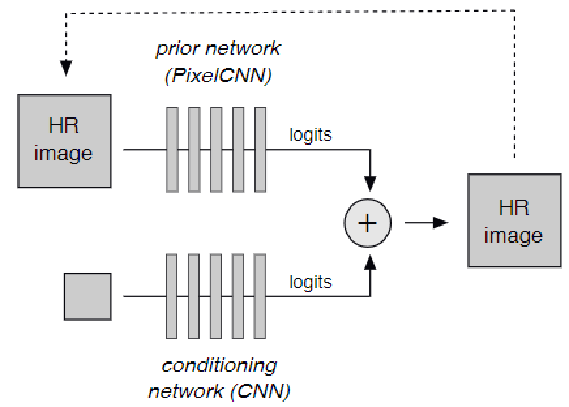
\includegraphics[width=0.4\textwidth]{figures/network}
    \caption{Conditional Gated pixelCNN模型示意图}
\end{figure}

\subsection{Conditioning Network}

根据我们的设计思想,Conditioning network的主要作用是为Prior network提供条件信息,我们所提供的条件信息是和目标预测同分辨率的图片。本论文的实现选用的是反卷积CNN,采用的反卷积CNN网络从一个$16\times 16$的输入开始,分别经过各若干的$1\times 1$卷积层,残差块(Residual Blocks),反卷积层,ReLU(Rectifier Linear Unit)激活层,残差块,$1\times 1$卷积层。

残差块是多层神经网络的堆叠,本文采用的残差块的具体结构是这样的:残差块总体分为5层,残差块第一层为$3\times 3$卷积层,采用same padding,第二层为批量规范化层(Batch Normalization),第三层为ReLU激活层,第四层与第一层的结构相同,第五层与第2层结构相同;整个残差块的输入进入到第一层$3\times 3$卷积层,输出为第五层批量规范化层和网络输入的直接融合;整个网络中,每一层的通道(Channel)数与输入的通道数相同。使用批量规范化层的效果是一方面保持前一层的特征图的数据均值,另一方面减少数据分布的弥散,保持一定的网络训练速度。

\begin{figure}[htp]
    \centering
    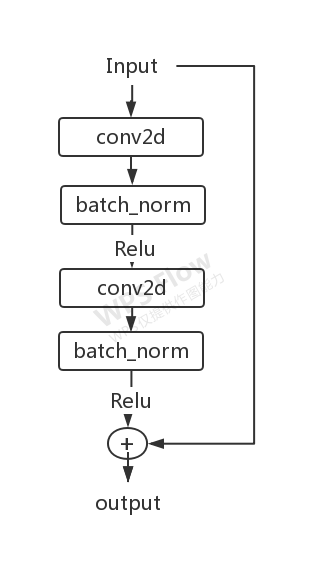
\includegraphics[width=0.2\textwidth]{figures/resnet}
    \caption{残差块结构示意图}
\end{figure}

本文采用的Conditioning network中包含这样一个结构:首先把输入送入$resnum$个残差块,再在残差块后接入一个反卷积层。在数据经过该反卷积层之后,输出特征图的分辨率为输入特征图的2倍。在这之后再接上一个ReLU激活层得到整个残差块的输出。我们将前述的包括残差块到ReLU激活层及其之间各层的多层神经网络堆叠称为一个\textbf{反卷积块(Deconvolution Block)}。

\begin{figure}[htp]
    \centering
    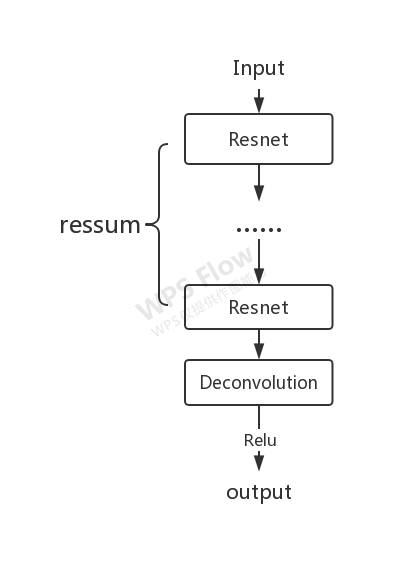
\includegraphics[width=0.3\textwidth]{figures/Deconvolution}
    \caption{反卷积块示意图}
\end{figure}

具体地,我们借助上文所述的几个概念来进一步阐述本论文采用的反卷积CNN的组织结构,其结构图如下所示:

%双栏图片
% \begin{figure*}[htp]
%     \centering
%     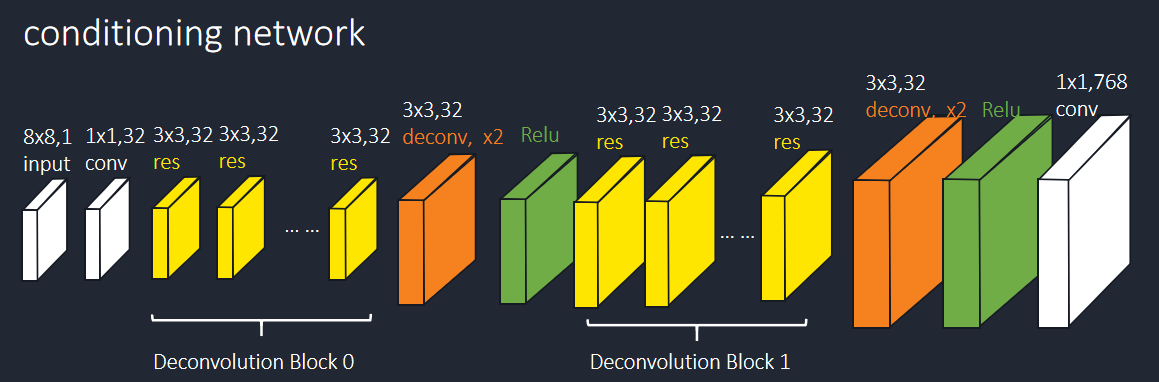
\includegraphics[width=0.8\textwidth]{figures/condition_network}
%     \caption{反卷积CNN结构示意图}
% \end{figure*}
\begin{figure}[htp]
    \centering
    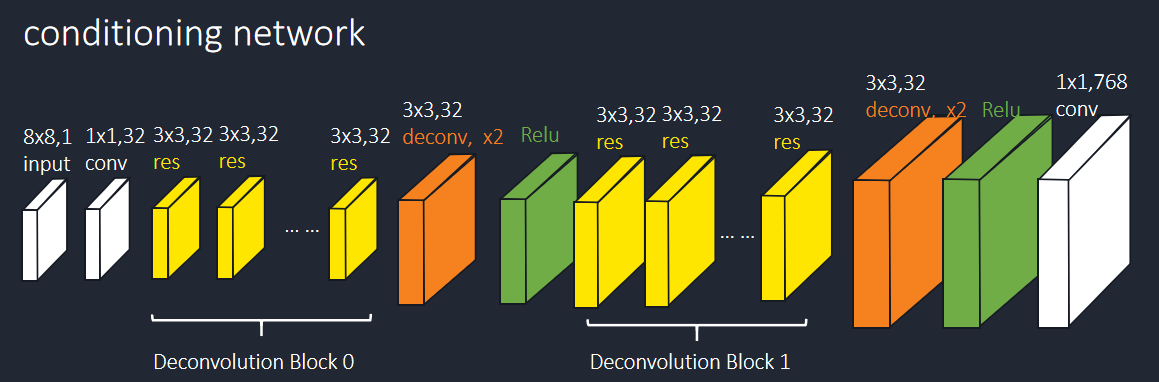
\includegraphics[width=0.5\textwidth]{figures/condition_network}
    \caption{反卷积CNN结构示意图}
\end{figure}

第一层$1\times 1$卷积层的主要作用是将channel数目增加到32个,达到数据升维的效果;而后堆叠两个反卷积块,此时网络大大加深的同时,在输出部分特征图的尺寸已经达到了$64\times 64$,而后接入$resnum$个残差块,最后以一个$1\times 1$卷积层结尾,网络通道数继续增加,达到$768$之多。整个Conditioning network在本实验中展现良好作用的关键点在于模型的:

\begin{enumerate}
    \item 残差块的运用使网络更深,数据内部表征更加丰富,训练效果更好。
    \item 反卷积层的使用,让网络的上采样过程变得可训练,有了更强的分辨率还原能力。
\end{enumerate}

因为Conditioning network和Prior network两者在逻辑上是可分的,因此我们在损失函数方面进行单独考虑,最后使用的是一个混合loss。根据Conditioning network的功能和输出,很自然地,我们希望Conditioning network的输出和标签越接近越好,因此Conditioning network这部分网络的损失函数采用的是数据标签和Conditioning network的输出的softmax loss。

\subsection{Prior network}

Prior network的设计定位是一个条件生成模型,其基本作用是学习如何从Conditioning network产生的条件概率,定向生成最终的图片。本文中的Prior network采用的是一个被称为Gated PixelCNN的模型结构,网络输入和输出都是$32\times 32$的特征图。为逐步阐述清楚Gated PixelCNN的设计思想,我们将逐步介绍Gated PixelCNN的灵感来源和发展。

Gated PixelCNN的灵感来源首先是PixelCNN。PixelCNN是一个像素级图像生成模型,其的结构和CNN尤其是FCN有许多类似之处,最大的区别在于卷积核方面。一个PixelCNN模型可以被很容易地拆分为重复层次的堆叠,其堆叠的一个基本单元我们称为一个\textbf{PixelCNN生成层}。

PixelCNN生成层使用Mask卷积核进行特征图处理,生成层的输入和输出都是一个特征图。Mask卷积核的结构就是在常规卷积核的基础上,增加一个Mask。在PixelCNN当中,有两种Mask,分别为A类Mask和B类Mask,其唯一区别在于,B类Mask的中心元素为1,而A类Mask为0。一个$5\times 5$的A类Mask的结构如图:

\begin{figure}[htp]
    \centering
    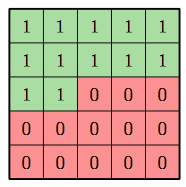
\includegraphics[width=0.3\textwidth]{figures/Mask结构.png}
    \caption{$5\times 5$A类Mask图示}
\end{figure}

在将该Mask与普通卷积核进行逐权重点积之后,再进行常规卷积操作。因为利用了前述的Mask卷积核,PixelCNN在生成当前位置像素的条件概率的时候,仅利用了在卷积核感受野中,处于当前像素位置之前的像素信息,而在当前像素之后的信息则被忽略。PixelCNN模型的算法训练过程中的优化目的是希望对每个标签像素计算到的概率都趋于1,而预测时,我们的Mask卷积核则生成关于颜色的概率密度函数,基于这个函数,我们为新像素填充概率最大的颜色,从而实现图像的生成。

以上就是PixelCNN的基本原理。

PixelCNN的图像生成效率较高,但生成图像素质却不如人意。因为其具有这样的缺点:

\begin{enumerate}
    \item PixelCNN因为受到阶梯状Mask的影响,在多层叠加时产生盲点,其中产生原因见下图
    \item PixelCNN本身建模能力较差
\end{enumerate}

其中盲点是因为PixelCNN在产生所需要的卷积核时,掩盖住了当前像素同一行的右边像素,当多层PixelCNN生成层堆叠时,因为叠加效应使得感受野产生了盲点。

\begin{figure}[htp]
    \centering
    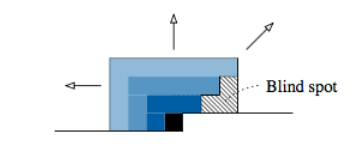
\includegraphics[width=0.3\textwidth]{figures/盲点产生.png}
    \caption{盲点产生图示}
\end{figure}

基于以上的考虑,本文采用了一种改进型的PixelCNN,被称为Gated PixelCNN。Gated PixelCNN为避免盲点问题,采用了改进的Mask卷积核,分为两部分:水平堆(Horizonta Stack)和垂直堆(Vertical Stack),其结构如图7所示。

\begin{figure}[htp]
    \centering
    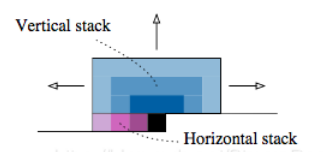
\includegraphics[width=0.3\textwidth]{figures/盲点的消除.png}
    \caption{Gated PixelCNN卷积核图示}
\end{figure}

卷积结果采用两个Mask卷积核的直接相加。因为两个部分的Mask都是矩形,经过堆叠依然是矩形结果,因此Gated PixelCNN就克服了原PixelCNN中产生的盲点问题。

因为需要的网络输出是每个像素的概率信息,因此Prior network采用Loss是Softmax Loss。

\subsection{Conditional Gated PixelCNN}

本论文采用Conditioning network和Prior network按照上文中基本结构进行结合,实现了我们Conditional Gated PixelCNN。PixelCNN本是一种具有随机性的生成模型,在本文中,通过引入Conditional Information,实现了生成模型的生成方向的控制,其中Conditional Information是由Conditioning network提供。

本文中的Conditional Gated PixelCNN的输出是Conditioning network和Prior network的直接叠加。采用的Loss方式是Softmax Loss,其取值等于两个网络模型单独Loss的直接相加。

我们选取这样的Loss以期结合的两个模型都能够得到恰当程度、比例的训练。




% \newpage
\section{实验}
\subsection{实验数据}
我们共使用了两个数据集对此模型进行了训练,一个为MNIST手写数字数据集,我们从中挑选出5k张label为'2'的图像进行训练;另一个为我们将多个数据集合并而成的亚洲人脸数据集,其中对各数据集中的图像进行了筛选工作如下:
\begin{enumerate}
\item CelebA开源名人人脸数据集\cite{liu2015deep},筛选出亚洲人脸图像4k张
\item AFAD开源亚洲年龄人脸数据集\cite{niu2016ordinal},筛选图像大小大于64×64,年龄在15-25岁之间,通过数字HIS处理亮度和对比度适中的图像4k张
\item CUHK证件照人脸数据集\cite{wang2008face},筛选大小适中的图像700张
\end{enumerate}
共计8700张图像作为亚洲人脸数据集。

由于Condition Network网络结构使得输入的低分辨率图像与生成的高分辨率图像的长宽之比均为1:4,因此我们使用双线性插值的方法对数据集进行处理,得到低分辨率图像为train data, 高分辨率图像为label。

为了更好地评判网络的预测效果,我们对不同的数据集切分得到不同的图像大小。对于MNIST数据集,低分辨率图像大小为7×7,高分辨率图像大小为28×28;对于人脸数据集,我们构建了8×8恢复到32×32以及16×16恢复到64×64两组实验来对网络进行训练。

\subsection{实验方案}
整个实验采取了在MNIST数据集上对模型进行调试,在亚洲人脸数据集上对模型进行评测的方案。

在模型评测的过程中,我们共构建了2组对照实验来检验网络模型的有效性,分别为8×8到32×32的图像恢复效果与16×16到64×64的图像恢复效果对照;只使用Condition Network的图像恢复效果与在Condition Network的基础上使用Prior Network的图像恢复效果对照。

\subsection{实验结果}
\subsubsection{MNIST数据集实验结果}
考虑到MNIST数据集图像简单且单一的特点,在MNIST数据集进行图像恢复时,仅使用Condition Network对模型进行训练,对参数进行简单调节后可达到一个较好的图像恢复效果。
\begin{figure}[htp]
    \centering
    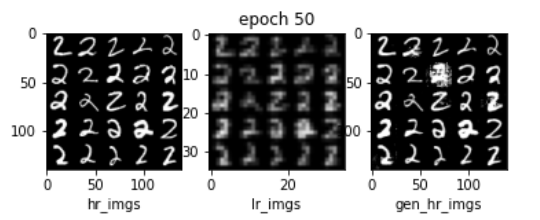
\includegraphics[width=0.46\textwidth]{figures/MNIST_all_epoch50}
    \caption{MNIST数据集 epochs = 50图像恢复结果}
    \label{MNIST_all_epoch50}
\end{figure}

如图 \ref{MNIST_all_epoch50}所示,当训练了50个epochs时,对大多数数字图像能恢复到可清晰辨识的状态,但对于少数图像的恢复效果不佳。

\begin{figure}[htp]
    \centering
    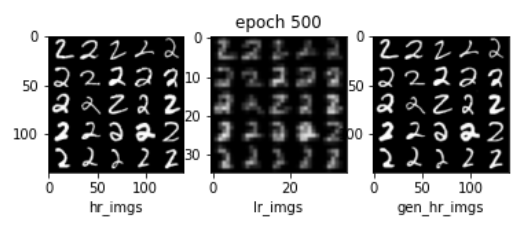
\includegraphics[width=0.46\textwidth]{figures/MNIST_all_epoch500}
    \caption{MNIST数据集 epochs = 500图像恢复结果}
    \label{MNIST_all_epoch500}
\end{figure}

\begin{figure}[htp]
    \centering
    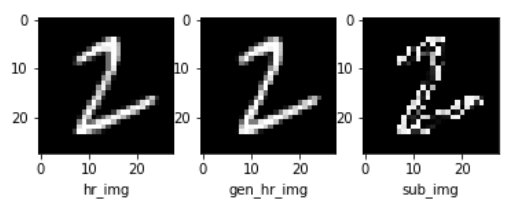
\includegraphics[width=0.46\textwidth]{figures/MNIST_sub}
    \caption{生成图像与原图的比较}
    \label{MNIST_sub}
\end{figure}

如图 \ref{MNIST_all_epoch500}、\ref{MNIST_sub}所示,当训练了1000个epochs时,模型的Loss下降到0.4以下,生成图与原图的差距较小,人眼几乎无法分辨。

\subsubsection{不同大小的图像恢复效果比较}
在对亚洲人脸数据集进行图像恢复时,我们进行了8×8图像恢复和16×16图像恢复两组实验,均只使用Condition Network进行图像恢复,并都对模型训练300epochs。

\begin{figure}[htp]
    \centering
    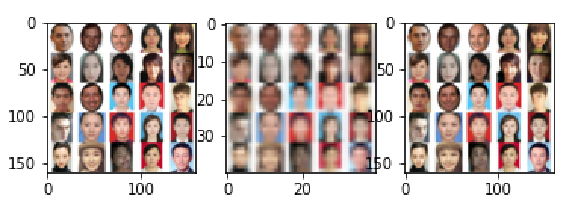
\includegraphics[width=0.46\textwidth]{figures/person_all_8}
    \caption{亚洲人脸数据集 8×8图像恢复结果}
    \label{person_all_8}
\end{figure}

\begin{figure}[htp]
    \centering
    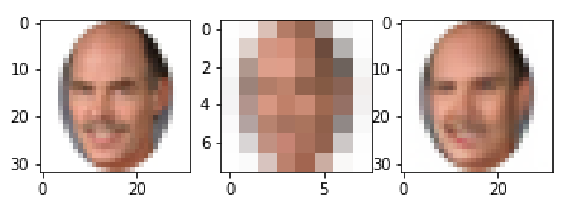
\includegraphics[width=0.46\textwidth]{figures/person_8}
    \caption{亚洲人脸数据集 8×8单张图像恢复结果}
    \label{person_8}
\end{figure}

从图\ref{person_all_8}、\ref{person_8}的图像恢复效果中我们发现,8×8的图像信息丢失严重,对于人眼来说已经很难辨识,而模型依旧能恢复出图像的大体轮廓。

\begin{figure}[htp]
    \centering
    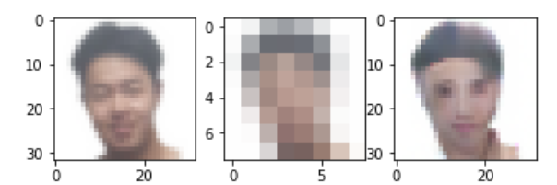
\includegraphics[width=0.46\textwidth]{figures/zzy_8}
    \caption{非正常角度的8×8图像恢复结果}
    \label{zzy_8}
\end{figure}

如图\ref{zzy_8}所示,此模型在细节上的恢复效果较差,尤其是对非正常角度拍摄的图像进行恢复时,会出现较严重的细节丢失现象,因此我们并不认为此模型在8×8这种超低分辨率的图像恢复上有较好的效果。

\begin{figure}[htp]
    \centering
    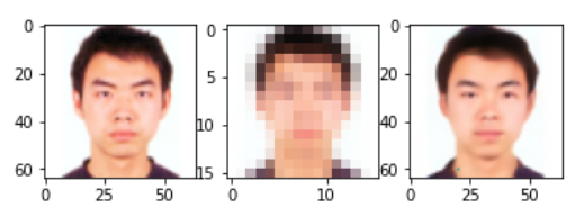
\includegraphics[width=0.46\textwidth]{figures/person_16}
    \caption{亚洲人脸数据集 16×16单张图像恢复结果}
    \label{person_16}
\end{figure}

从图\ref{person_16}中可以看出,相较于8×8图像恢复而言,16×16图像恢复在细节处理上效果更好,并且由于低分辨率图所包含的信息更大,所以图像恢复的泛化能力更强,对非正常角度的图像也有一定的回复能力。因此我们更倾向于以16×16图像恢复的效果来对我们的模型进行评价。

\subsubsection{是否使用prior network的图像恢复效果比较}
在对16×16的图像恢复的基础上,我们对Prior Network网络进行了评测,在有无Prior Network的情况下,图像恢复效果也不同。

在实验中我们发现,Condition Network与Prior Network两个网络分开训练与协同训练的图像恢复效果差别并不大。为了更公正的评测Prior Nwtwork的图像恢复效果,我们选择了两个网络分开训练的方式,以此保证了在对照实验中,Condition Network的训练效果一致,对图像恢复效果差异不造成影响。

\begin{figure}[htp]
    \centering
    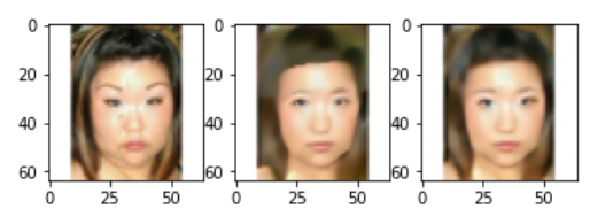
\includegraphics[width=0.46\textwidth]{figures/prior}
    \caption{是否使用Prior Network的图像恢复效果比较}
    \label{prior}
\end{figure}

如图\ref{prior}所示,相较于仅使用Condition Network的图像恢复结果而言,使用Prior Network会使得恢复出的图像在许多细节上获取到一种整体特征,比如在发型轮廓上,Prior Network会使得图像的这一部分更加真实,当然也是更接近于整体平均水平。

\subsubsection{图像恢复的局限性与泛化能力}

\begin{figure}[htp]
    \centering
    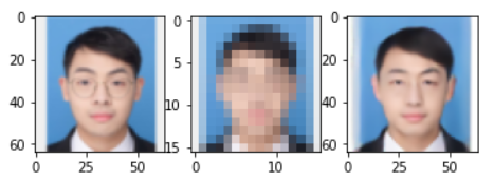
\includegraphics[width=0.46\textwidth]{figures/ly}
    \caption{戴眼镜的人物图像恢复}
    \label{ly}
\end{figure}

如图\ref{ly}所示,使用此模型进行图像恢复极其受限于数据集,当需恢复的图像包含有数据集不包含的特征(例如眼镜、胡须、辫子等)时,恢复效果会较差。

\begin{figure}[htp]
    \centering
    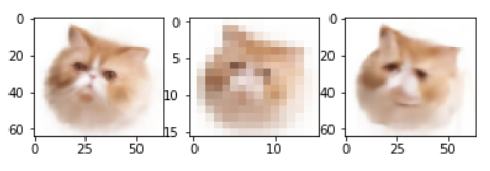
\includegraphics[width=0.46\textwidth]{figures/cat}
    \caption{非人类的人物图像恢复}
    \label{cat}
\end{figure}

如图\ref{cat}所示,当对非人类图像进行预测时该模型也有一定的预测效果,一方面说明模型并未过拟合,另一方面说明该模型具有一定的泛化能力,能够较为准确地提供一种对各类图像的恢复方案。

\subsection{图像相似性的定量评估}
对图像相似性的量化方法有很多,最常见的有均方误差MSE, 结构相似性SSIM, 以及峰值信噪比PSNR三种,我们在实验中使用到的图像相似性量化标准为均方误差MSE。

\begin{figure}[htp]
    \centering
    
\includegraphics[width=0.46\textwidth]{figures/mse}
    \caption{均方误差MSE}
\end{figure}

\subsection{对人类的感知评估}
在误差分析过程中我们发现,定量的方式实际上与人类的感知判断并不完全相符,很多看起来恢复效果不佳的图像却定量评估上表现较好。因此在后续的调节过程与最终的模型效果评判上,我们更多地参考了人类的感知来对模型进行调整与评价。


\section{结论}

基于Gated Pixcnn图像重建是一种完全基于概率的图像恢复方法,该方法只需要较少的训练集即可达到一个还算不错的图像超分辨率重建效果,但在细节部分表现不佳。并且该模型具有较强的泛化能力,能够胜任各类图像的超分辨率重建,尤其适用于对细节不敏感的图像重建。

本文具体讲述了基于Conditional Gated PixelCNN的图像超分辨率重建技术的实现方法与实验效果,除了一般的回归模型外,并未与业内的其他模型进行比较,在后续的工作中,可以将该模型与GAN模型进行效果比较。在对模型的定量评估上,本文采用的是自定量的评估标准,而这种标准可能是不符合人类感知的,在后续的工作中,可以在更大的范围里以人类的感知来对模型的图像重建效果进行评价。

% \newpage
\section{计算机学报的模板}
对投稿的基本要求:

\begin{theorem}
  定理内容。
  “定义”、“假设”、“公理”、“引理”等的排版格式与此相同,详细定理证明、公式可放在附录中。
\end{theorem}

\begin{proof}
  证明过程.
\end{proof}


\begin{table}[htb]
  \centering
  \caption{表说明}
  \small
  \begin{tabular}{cc}
    \toprule
    示例表格 & 第一行为表头,表头要有内容 \\
    \midrule
    & \\
    \midrule
    & \\
    \bottomrule
  \end{tabular}
\end{table}

\begin{procedure}
  \caption{过程名称}
  \small
  \begin{algorithmic}
    \REQUIRE
    \ENSURE
    \STATE \COMMENT{《计算机学报》的方法过程描述字体为小5号宋体,IF 、THEN等伪代码关键词全部用大写字母,变量和函数名称用斜体}
  \end{algorithmic}
\end{procedure}

\begin{algorithm}
  \caption{算法名称}
  \small
  \begin{algorithmic}
    \REQUIRE $n \geq 0 \vee x \neq 0$
    \ENSURE $y = x^n$
    \STATE $y \leftarrow 1$
    \IF{$n < 0$}
      \STATE $X \leftarrow 1 / x$
      \STATE $N \leftarrow -n$
    \ELSE
      \STATE $X \leftarrow x$
      \STATE $N \leftarrow n$
    \ENDIF
    \WHILE{$N \neq 0$}
      \IF{$N$ is even}
        \STATE $X \leftarrow X \times X$
        \STATE $N \leftarrow N / 2$
      \ELSE[$N$ is odd]
        \STATE $y \leftarrow y \times X$
        \STATE $N \leftarrow N - 1$
      \ENDIF
    \ENDWHILE
  \end{algorithmic}
\end{algorithm}


\begin{acknowledgments}
  感谢王兴刚老师对本篇论文工作的悉心指导和提出的宝贵建议。
\end{acknowledgments}

\appendix

\section{人员分工}
\begin{table}  
    \begin{center}  
    \begin{tabular}{|l| m{5cm}|}  
    \hline  
        刘羿 & 选题调研、Condtional Network设计与实现、Prior     Network设计与实现、服务器模型训练自动化、开题PPT制作与汇报、结题PPT制作与汇报、最终论文撰写 \\ \hline
        张志宇 & 选题调研、相关文献调研、论文复现、数据集获取、Prior     Network设计与实现、服务器模型训练自动化、开题PPT制作与汇报、结题PPT制作与汇报、最终论文撰写\\ \hline  
        李勉 & 选题调研、相关文献调研、论文复现、数据集获取、服务器模型训练自动化、结题PPT制作与汇报、最终论文撰写 \\ 
    \hline  
    \end{tabular}  
    \end{center}
    \caption{人员分工}  
\end{table}

\nocite{*}
\bibliographystyle{cjc}
\bibliography{ref}

\newpage

\makebiographies


% \begin{background}
% *论文背景介绍为英文,字体为小5号Times New Roman体*

% 论文后面为400单词左右的英文背景介绍。这是我们的介绍:

% 本文研究的问题属于哪一个领域的什么问题。该类问题目前国际上解决到什么程度。

% 本文将问题解决到什么程度。

% 课题所属的项目。

% 项目的意义。

% 本研究群体以往在这个方向上的研究成果。

% 本文的成果是解决大课题中的哪一部分,如果涉及863/973以及其项目、基金、研究计划,注意这些项目的英文名称应书写正确。
% \end{background}

\end{document}
